\section{Preliminaries}

\subsection{Choosing a DBMS}
\label{sec:dbms}

For the choice of a suitable database management system underlying the
core translation memory and the user space, the main points we
considered were

\begin{itemize}
\item
  software license of the DBMS
\item
  general performance and maintainability
\item
  included support for fuzzy matching and custom indexes
\end{itemize}
According to these requirements, we evaluated several database systems
and selected the open source database system
PostgreSQL.\footnote{\url{http://www.postgresql.org/}} This system
fulfills the requirements as follows:

\begin{itemize}
\item
  open license similar to BSD license
\item
  good results in performance evaluations and good reputation for
  maintainability
\item
  support for phonetic representation of strings (SOUNDEX and
  METAPHONE), string edit distance (Levenshtein), fuzzy string search
  using character trigrams and customizable indexes (GIST, GIN)
\end{itemize}

For managing connections to the database in Java and Scala, we use JDBC, 
which allows the database connection to easily use another DBMS. 
In the XML-based configuration file (see the user's manual), the JDBC connector
and username and password to the database have to be specified. When testing the
translation memory with project-internal unit tests, we replace the production JDBC
configuration with a temporary in-memory database (HSQLDB\footnote{\url{http://hsqldb.org/}}).

\lstset{language=XML, caption={Configuration }}
\begin{lstlisting}
<database>
    <connector>jdbc:postgresql://localhost/filmtit</connector>
    <user>postgres</user>
    <password>postgres</password>
</database>
\end{lstlisting}

\section{Architecture of the Core Translation Memory}

The core translation memory consists of the database of chunks and media
sources (movies and TV shows) which are indexed in several ways for fast
retrieval. A query to the translation memory generally proceeds in two
steps: In a first step, translation pairs for a chunk are retrieved from
the database. The second step consists of ranking the candidates
retrieved in the first step according to their quality and how well they
match the query. If the quality of the retrieved candidates exceeds a
minimum quality threshold, they will be sent to the user.

\subsection{Backoff translation memories}

The idea of a backoff translation memory is to use multiple ways of
retrieving and ranking candidate translation pairs from the database and
``back off'' to a less exact level of retrieving and ranking when there
are no satisfactory results on the current level.

A backoff translation memory consists of a \emph{translation pair
searcher}, a \emph{translation pair ranker}, a \emph{minimal quality
threshold}, and another optional \emph{backoff translation memory}. If
the results retrieved by the \emph{searcher} and ranked (and scored) by
the \emph{ranker} do not meet the threshold, then the query is sent to
the backoff translation memory. The backoff translation memory can
itself be backoff translation memory.


\section{Candidate retrieval}
\label{sec:candidate_retrieval}

We implemented several methods for efficiently retrieving candidate
translation pairs from the database. The most general method
is the usage of an indexed signature strings. In this method, for each
chunk stored in the database, a string is produced by a signature
function and this string is used as an index for the database relation.
Several signature functions are used in the translation memory
implementation. Within the database, each signature function is represented by 
a relation which is indexed by the signature and refers to the original
translation pair.

\begin{figure}[h!]
	\centering
		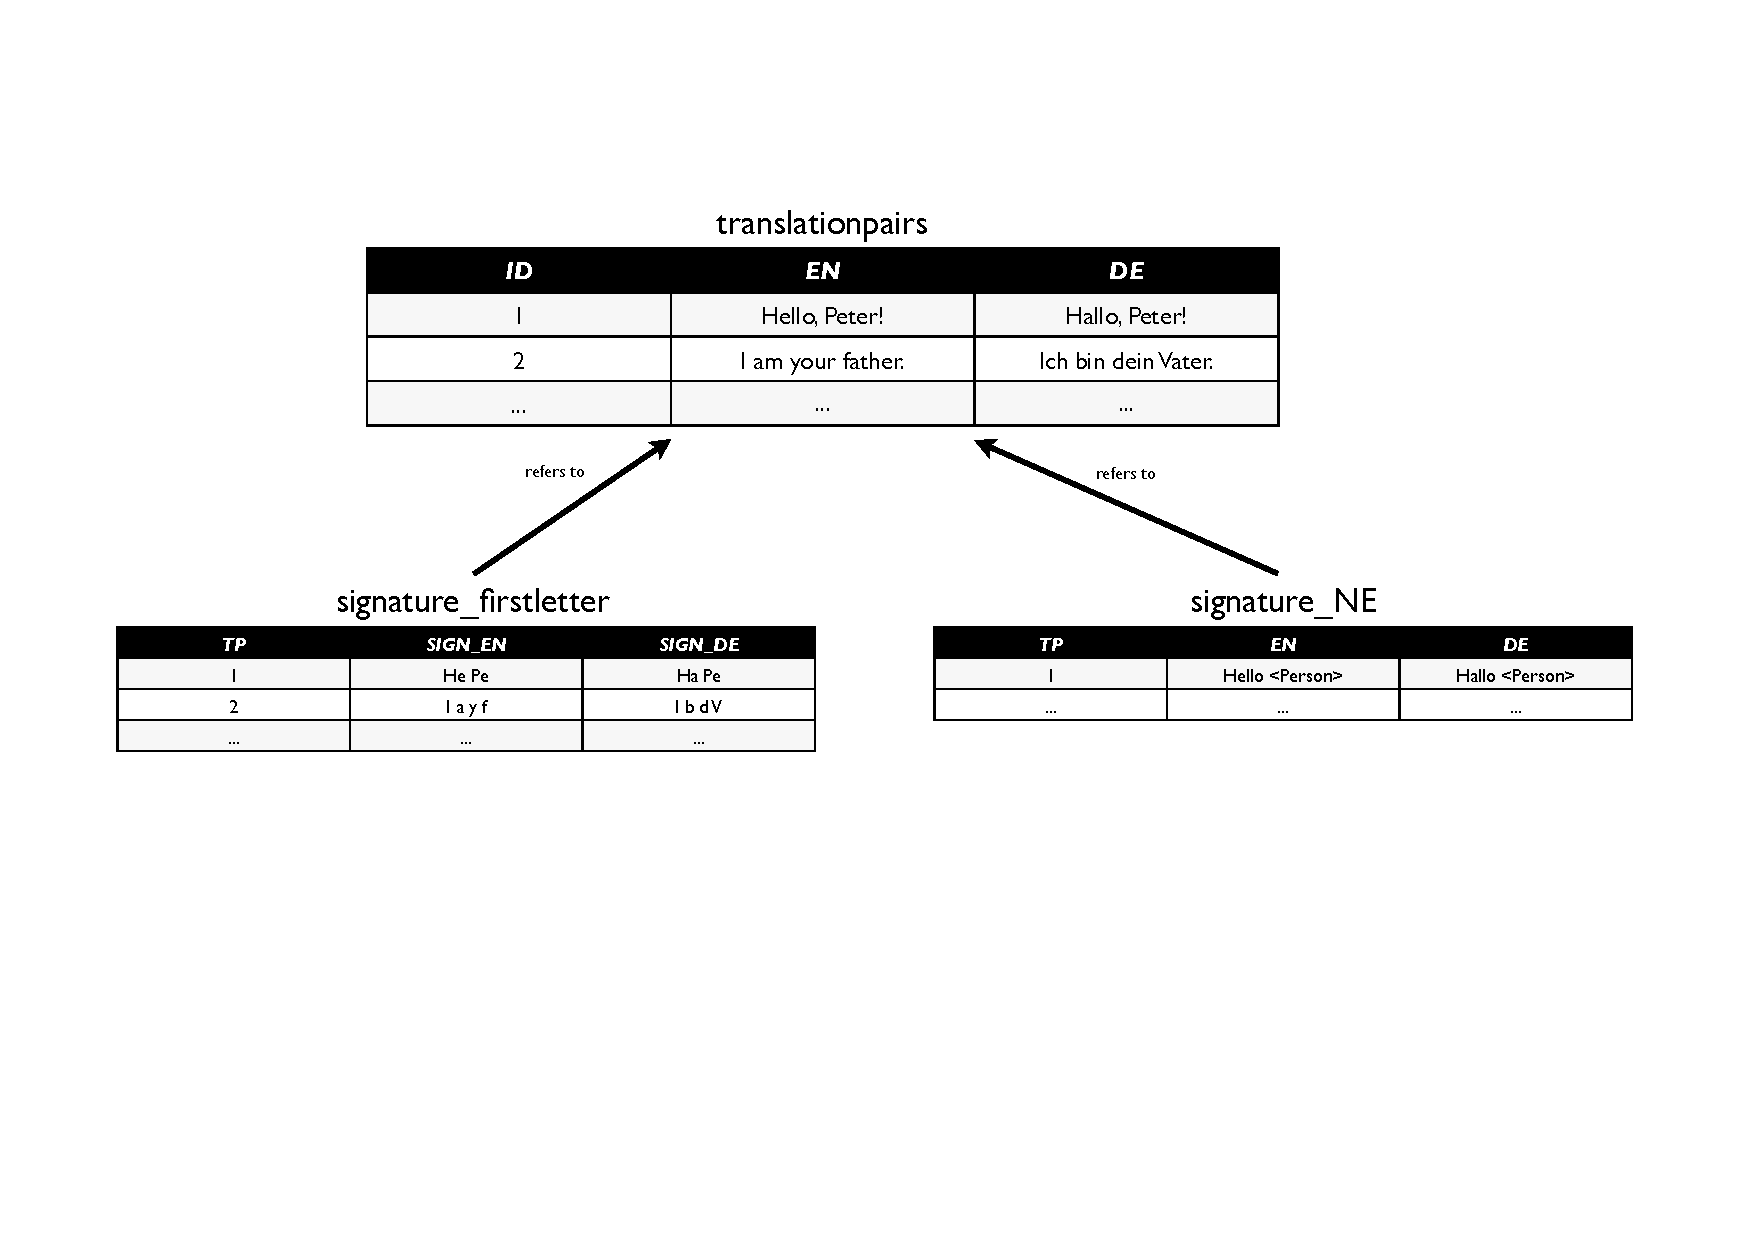
\includegraphics[width=17cm]{figures/core/signatures.pdf}
	\caption{Illustration of signature strings in the database.}
	\label{fig:figures_core_signatures}
\end{figure}

In the following sections, the signature functions will be illustrated.

\newpage
\subsection{Tokenization}

For all retrieval methods, we tokenize, i.e. separate the input sentence into individual tokens,
all inputs using tokenizers provided by the Apache OpenNLP project.\footnote{\url{http://opennlp.apache.org/}}
OpenNLP provides both unsupervised and supervised methods of tokenization. 
As a default tokenizer, we use an unsupervised tokenizer that splits the input
based on white space. This method has the advantage that is applicable to any new
language without requiring further training, however the result is of moderate
quality and often leads to problems in latter processing steps (e.g. Named Entity Recognition).

To improve the results, we use a Maximum-Entropy based OpenNLP tokenizer. For English, we use the
models provided by the OpenNLP project. For Czech, no such model existed, so we trained a ME tokenizer
model on data from the Prague Dependency Treebank\footnote{\url{http://ufal.mff.cuni.cz/pdt2.0/}}.\\

\noindent For training the ME tokenizer, we produced a script that creates training data in the following format:
\lstset{caption={Example training data for OpenNLP ME tokenizer.}}
\begin{verbatim}
K vynikajícím spisovatelům<SPLIT>, kteří věřili v nevysvětlitelné duševní 
úkazy<SPLIT>, patřil také americký romanopisec Upton Sinclair<SPLIT>.
\end{verbatim}

In the training data, the \verb|<SPLIT>| annotation indicates a position in the data, in which the
tokenizer is required to separate two tokens (in this case words and punctuation symbols). These
positions were manually marked in the Prague Dependency Treebank by annotators.

On a test dataset from the Prague Dependency Treebank, the ME tokenizer achieved the following results:

\begin{lstlisting}
Precision: 0.9970180340649772
Recall: 0.9954658318039512
F-Measure: 0.9962413283293529
\end{lstlisting}

%TODO: layout this (table or something)



\subsection{Signature-based retrieval: Exact matches}

The first signature function is for retrieving exact matches. For this,
the signature function consists of the first letters of each word in the
chunk. Punctuation is dropped from the signature. If the queried chunk is
very short, only using the first letter would produce a very high number of
results. Hence, for short chunks, more letters of each individual token are
included.



\subsection{Signature-based retrieval: Named Entities}

The second, more fuzzy signature function uses named entity recognition
to provide matches. Named entity recognition is the task of finding
elements in a text belonging to basic name categories like
\emph{Person}, \emph{Organization} and \emph{Place}. In the signature,
the surface form of the named entity is replaced by its named entity
category. This allows the retrieval of candidate chunks that differ only
in the named entities they are using. As an example, consider the
following chunks:

\begin{lstlisting}
Chunk 1:   Peter saw the girl.
Signature: <Person> saw the girl

Chunk 2:   Thomas saw the girl.
Signature: <Person> saw the girl
\end{lstlisting}

Using the named entity-based signature, Chunk 2 can be retrieved as a
candidate for chunk 1. Since an exact match would be preferable, this 
will only be used if there is no better fitting candidate in the
database.

\subsubsection{Named Entity Recognizers}

For Named entity recognition, we use the OpenNLP Maximum Entropy based
Named entity recognizers. For English, we were able to use the pre-trained
models for persons, organizations and places that are available through the
OpenNLP project.

For Czech, no such models were available, hence we trained our own models based
on various data sources and then chose the best models from the comparison 
of two approaches of acquiring training data.


\subsubsection*{First approach: Training data based on Wikipedia and DBpedia}

Our first approach to acquiring named entity recognition training data for Czech 
was based on the Pig NLProc utility\footnote{\url{https://github.com/ogrisel/pignlproc}}.
Pig is an Apache project providing platform that features a SQL-like syntax
for data analysis based on Apache Hadoop. The Pig NLProc utility provides a number
of Pig scripts to extract natural language processing training data from Wikipedia
and DBpedia.

DBpedia is a \footnote{\url{http://dbpedia.org/About}} community project for extracting 
structured data from Wikipedia. Based on user-created mappings of Wikipedia info boxes to
an ontology, DBpedia provides data that allows to easily select DBpedia entites that 
correspond to persons, organizations, places, etc.

To acquire named entity recognition training data, the Pig NLProc utility searches
for article references to Wikipedia pages that are known (from the DBpedia ontology)
to be of the required types (e.g. Person). These instances are sentences with links
to the given article and these are then converted to the training format required 
by OpenNLP.

For Czech, user-generated mappings for many info boxes are already available, however,
the DBpedia data for Czech is not yet available. Hence, we downloaded the DBpedia
extraction framework with the Czech data and ran the extraction process ourselves.
With the resulting data and the Pig NLProc scripts (which required minimal changes
for issues of compatibility), we produced training data for named entities of the types
Person, Place and Organization.



\subsubsection*{Second approach: Training data based on the Czech Named Entity Corpus}

The second approach is based on the Czech Named Entity corpus.\footnote{\url{http://ufal.mff.cuni.cz/tectomt/releases/czech_named_entity_corpus_10/index.html}}
The corpus contains manual named entity annotations of a large number of named entity types. Figure~\ref{fig:figures_core_CzechNECorpus}
shows an overview of the NE types annotated in the corpus.


\begin{figure}
	\centering
		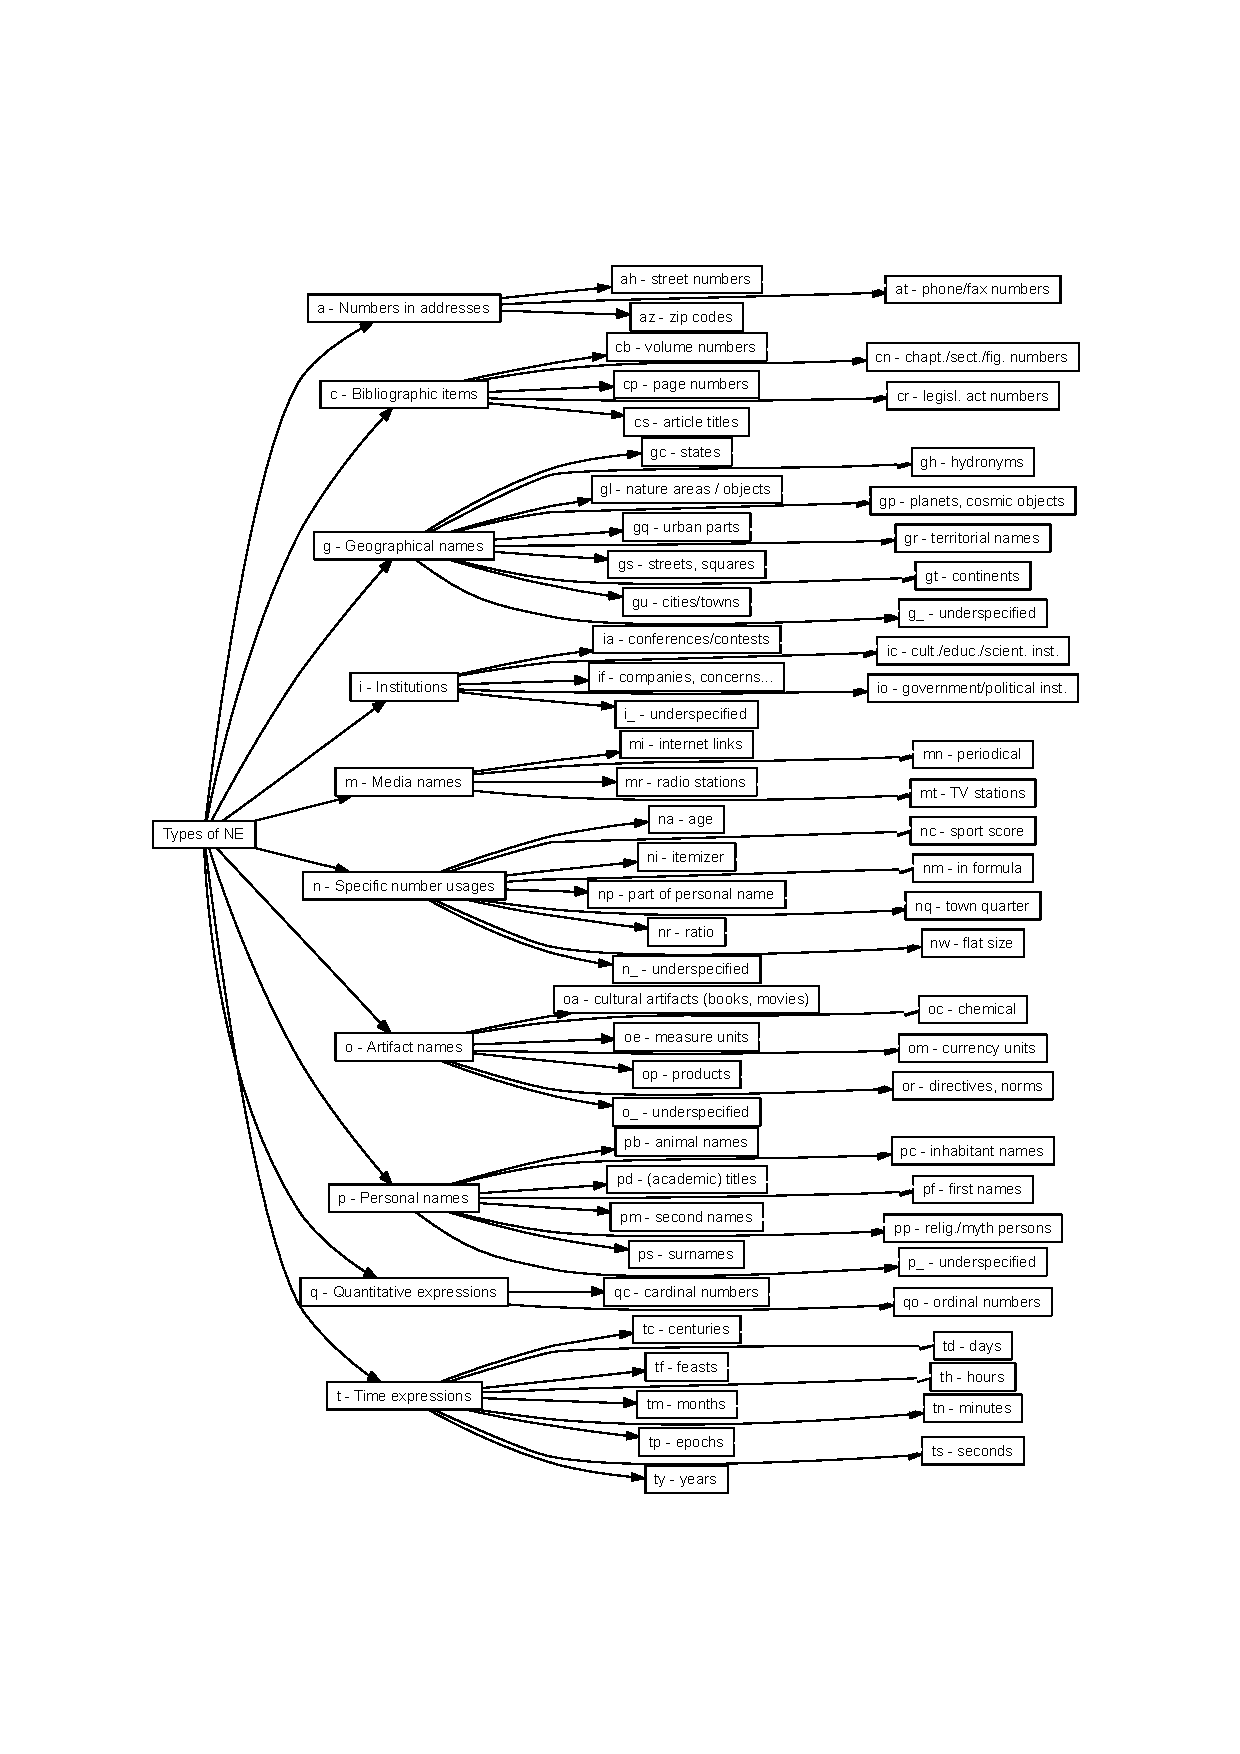
\includegraphics[width=16
		 cm]{figures/core/CzechNECorpus.pdf}
	\caption{Named entity types in the Czech Named Entity corpus. Source: Czech Named Entity corpus documentation.}
	\label{fig:figures_core_CzechNECorpus}
\end{figure}


We wrote scripts that convert the XML-based format of the corpus to the format required by OpenNLP, 
manually selected the annotation types and trained the OpenNLP named entity recognizers on the resulting data.


\subsubsection*{Selecting the best approach}

Both approaches showed to have their unique advantages and disadvantages. While the first approach is only minimally supervised
and can easily be extended to other languages that have a local version of Wikipedia and existing DBpedia dumps (DBpedia dumps are currently available for 97 languages\footnote{\url{http://wiki.dbpedia.org/Downloads37}}), our manual evaluation of the produced Named Entity recognizers showed that the models trained on the Czech Named Entity corpus produced better results.

More precisely, we approximated, that the DBPedia recognized far less cases and, therefore, had much lower RECALL, the PRECISION was only slightly better. We then decided, that lower RECALL is worse for our purposes -- it's better to show wrong translation to user than to not show anything.

\subsubsection*{Effectiveness}
It's worth noting that the overall effectiveness of using named entity-based retrieval was worse than we anticipated. In most subtitles, there is not a single match, but the recognition of named entities takes the most time during the data import.  

TODO:DATA HERE

\subsection{External services}

As another backoff level, we use Machine Translation from external services.
For this, a query with the chunk is sent to an external REST-based
API.\footnote{We use the free Machine Translation API of the MyMemory project, cf. \url{http://mymemory.translated.net/doc/spec.php}.}
If the resulting translation meets the minimal quality threshold, it
will be presented to the user.

However, there is no machine translation service with unlimited free REST-based API, and, for example, MyMemory project has so low daily quota, that we get over its quota with averagely TODO:FILLDATA subtitle files.

\subsection{Statistical Machine-Translation based on Moses}




\section{Candidate Ranking}

After retrieving candidates for a query, the candidate translation pairs must be ranked according to their quality and how well they fit the query. We use different methods for ranking the candidates retrieved by the candidate retrieval methods.


\subsection{Ranking for exact matches}

For exact matches, 


\section{Merging similar candidates}




\section{Technical issues}

\subsection{Concurrency}





\subsection{Keeping the database up to date}




